\chapter{基于鞅保护分布方法的无人机集群行为分类研究}
\label{chapter:swarm-martingales}
\section{引言}
第\ref{chapter:swarm-distributions}章的结论表明实际工程数据自身的时间顺序是很重要的信息。在处理实际工程问题时, 不能轻易通过技术随机打乱实际工程应用中数据本身的时间信息。同时, 第\ref{chapter:swarm-distributions}章的结论也表明, 当按照数据本身时间顺序构建机器学习模型时, 模型的预测能力通常是有限度的。为提高实际工程问题中模型预测效果, 本章提出一种融合数据本身时间顺序的方法, 这种方法仍然是建立在底层机器学习算法之上的, 因此本章提出的算法依旧可以提升机器学习算法的预测效果。

第\ref{chapter:swarm-distributions}章的结论同时也表明随机化能够明显提高机器学习模型的预测效果。因此, 本章将第\ref{chapter:swarm-distributions}章研究的结论综合起来考虑: 本章中仍然处理实际工程应用中的有序学习问题, 虽然数据本身的时间顺序无法随机化, 但是本章可以为模型提供一种随机化方案, 即将模型中最外层具有固定形式的函数随机处理。本章仍然采用一致性预测思想实现这一目的。

\section{基于一致性预测的鞅保护分布方法理论研究}
\label{transductive}

本章围绕为考虑数据自身时间顺序的无人机集群数据展开高效的行为分类。 首先对于无人机集群行为分类问题, 将之归约为模式识别问题。正如第\ref{chap:edbed}章已经阐明的, 对于模式识别问题, 其基本假设是给定训练样本数据集由固定的、但未知的概率分布函数独立地生成。基于经验数据, 学习器在诸函数的集合——这些诸函数是由机器实现的——中挑选一个函数 $f(x, \alpha_{0})$, 此函数能够最小化错误分类数目。 目前的大多数机器学习方法都基于此问题假设, 形成一种离线学习框架。 使用一批学习样本得到某规则函数, 进而将规则函数应用于测试样本。 这样的工作在集群学习领域已经有众多的研究文献。 例如, \citet{Brown2014} 基于受限带宽情形下利用机器学习算法识别集群行为分类; \citet{Berger2016}提出一种压缩子空间的方法实现集群行为分类方法; \citet{Thomas2021}则将集群整体看做动态系统来揭示集群行为所产生的影响。

然而, 由于本章考虑按照实际工程中数据本身的时间顺序预测无人机集群行为, 因此需要针对有序学习展开讨论。保留实际数据自身时间顺序的有序学习属于超越推理范式\citep{vapnik1995,vapnik1998}。 超越推理是由Vapnik提出的一种新的学习范式, 这种学习范式考虑为保留时间顺序的真实数据提供预测估计。在技术层面而言, 与超越推理对应的传统统计学基于归纳推理范式。归纳推理范式需要两步完成推理, 首先需要估计一般函数参数, 然后再将新观测数据输入估计函数得到预测值\citep{Fisher1956}。 与此相反, 超越推理利用经验数据直接得到对应的函数的值, 这种推理范式由于和实际工程问题高度匹配, 近些年受到越来愈多研究者的关注\citep{Becker2014,Luc2014}。也就是说, 根据超越推理范式, 观测到第一个对象$x_{1}$后开始预测对应的标签$y_{1}$; 然后观测到第二个对象$x_{2}$后开始预测其标签$y_{2}$, 以此类推。因此在这种推理范式下不允许研究者提前随机化数据。

由于在超越推理范式下无法随机化数据, 因此数据本身无法满足独立同分布的假设条件, 所以在处理实际问题时总会遇到分布漂移的问题。同时经过第\ref{chapter:swarm-distributions}章的研究已经表明, 实际工程数据自身的时间顺序是很重要的信息。为此, 本章提出一种将数据本身时间顺序纳入底层机器学习算法来增强底层机器学习算法的泛化推广能力。

\subsection{鞅保护分布方法研究现状}
考虑数据本身时间顺序的研究主要由Vovk提出。可以采用各种不同的分布漂移解决方案提升机器学习的学习能力。例如, \citet{Vovk2021retrain}提出通过鞅序列检测理论给出的分布漂移位点指示, 当鞅序列取值大于给定阈值时, 可以对学习模型进行二次训练以提升预测性能。但是则从另一个角度出发, 通过将考虑数据本身时间顺序的鞅序列融合至底层算法, 这样就无需二次训练而直接提升底层算法的预测效果。\citet{Vovk2021protectedregression}首次提出基于一致性预测的鞅保护分类方法, 并首先将之应用于处理回归问题。同样的\citet{Vovk2021protectedclassification}后来将提出的基于一致性预测方法的鞅保护分布方法应用于分类问题。 注意到这项工作后, 便将之引入无人机集群行为分类研究领域, 以期通过鞅保护分布的分类方法来提升有序学习时机器对复杂无人机集群行为的辨识能力。 

鞅保护分布算法的优点在于其可以作用于机器学习算法顶层, 通过对机器学习算法的输出——称之为暴力得分函数——进行鞅保护分布方法校正以获得更好的预测能力。因为受到底层机器学习算法的支撑, 这种方法可以克服“维数灾难”问题, 能够处理任意的超高维问题。图\ref{fig:align-example}展示鞅保护SVMs算法和鞅保护神经网络算法与无保护措施SVMs算法和无保护措施神经网络算法在预测问题上的对比, 模型的预测效果采用ROC曲线作为评价指标。图\ref{svm-1} 展示的是鞅保护SVMs算法的提升效果, 从图中可以看到未经鞅保护分布算法的SVMs算法预测的ROC曲线面积——即AUC值——为0.654, 经过鞅保护分布算法提升后其预测AUC值提升为0.734; 图\ref{nn-1} 展示的是鞅保护神经网络算法的提升效果, 从图中可以看到未经鞅保护分布算法的神经网络算法预测的AUC值为0.517, 经过鞅保护分布算法提升后其预测AUC值提升为0.724。图\ref{fig:align-example}给出的例子说明鞅保护分布算法能够明显提升底层机器学习算法的预测能力。

本章首先介绍鞅保护分布算法的理论, 然后将提出的鞅保护分布算法应用于处理无人机集群行为分类问题, 构建无人机集群鞅保护分布算法, 形成一套端到端的并且可建立在机器学习算法顶层的鞅保护分布框架。 因为引入鞅保护分布后数据本身的时间顺序得到考量, 因此对于实际工程中遇到的真实数据分析任务能够提供相当可观的提升效果。

%\begin{figure*} % [tb]
%\begin{center}
%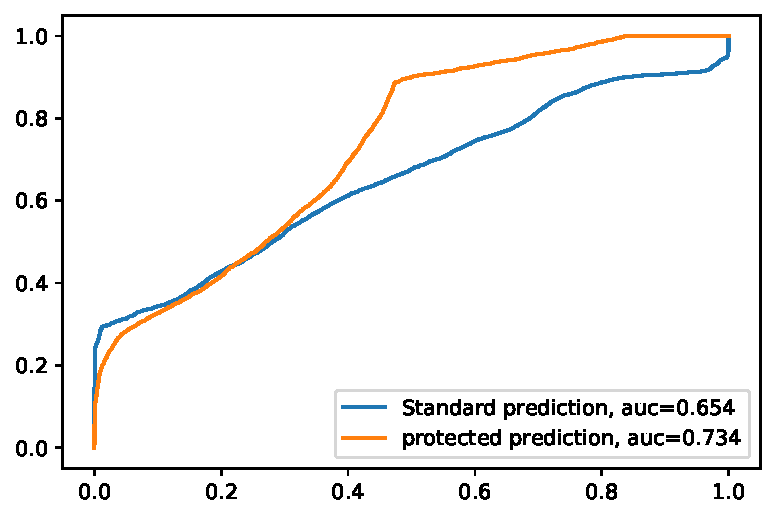
\includegraphics[scale=.5]{Img/chapter11/align-SVC}
%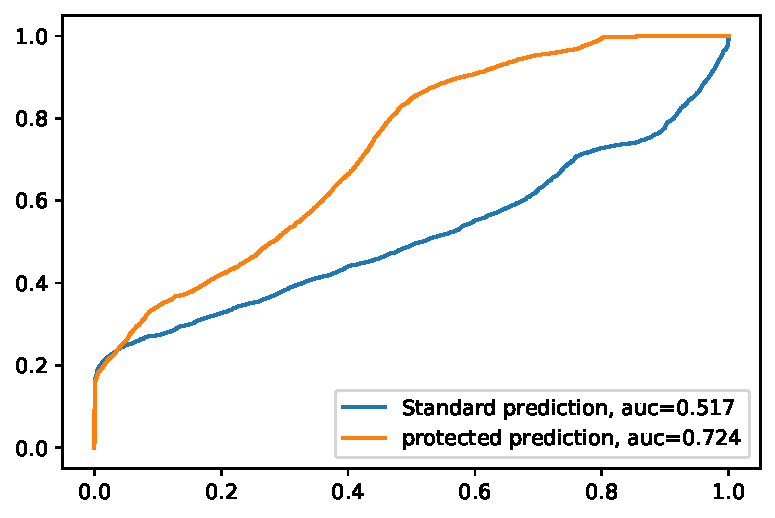
\includegraphics[scale=.5]{Img/chapter11/align-MLPClassifier}
%\end{center}
%\caption{鞅保护SVMs和鞅保护神经网络算法分类结果示例}
%\label{fig:align-example}
%\end{figure*}
%

\begin{figure}
     \centering
     \begin{subfigure}[b]{.45\textwidth}
         \centering
         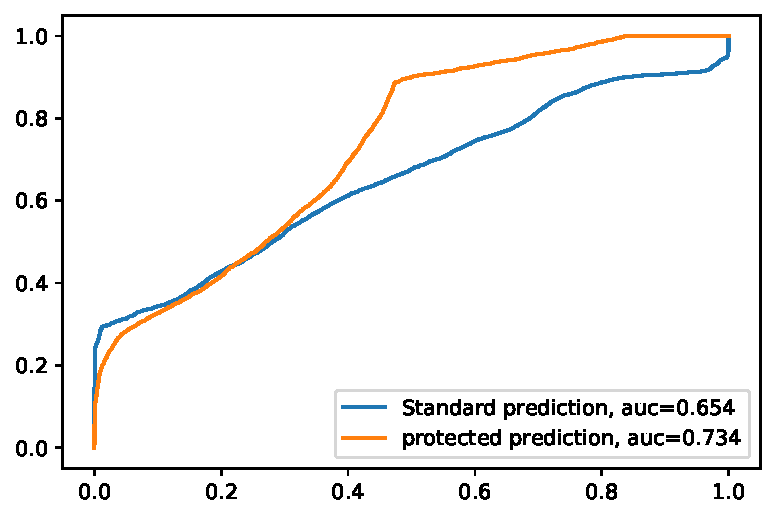
\includegraphics[width=1\textwidth]{Img/chapter11/align-SVC}   
         \caption{SVMs鞅保护算法分类结果}
         \label{svm-1}
     \end{subfigure}
     \hfill
     \begin{subfigure}[b]{.45\textwidth}
         \centering
         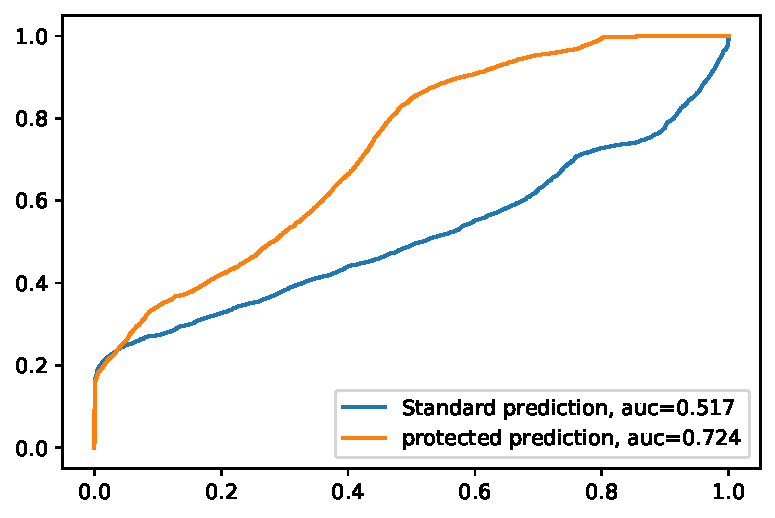
\includegraphics[width=1\textwidth]{Img/chapter11/align-MLPClassifier}
         \caption{神经网络鞅保护算法分类结果}
         \label{nn-1}
     \end{subfigure}
\caption{鞅保护SVMs和鞅保护神经网络算法分类结果示例}
\label{fig:align-example}
\end{figure}

\subsection{鞅保护分布方法理论研究}
本节介绍鞅保护分布方法的理论。根据第二章研究的VC理论, 学习机器推广泛化能力的控制是由两个因素决定的, 即不仅仅需要控制训练误差, 而且需要控制容量$h$。 通过鞅保护分布方法可以提升学习器的推广泛化能力, 此方法通过随机化模型最外层函数的具体形式, 将单一函数转变为“模糊函数带”来实现目标, 这相当于增加函数的丰富程度。


为实现在VC理论指导下鞅保护分布算法泛化推广能力的控制, 根据第\ref{chapter:swarm-distributions}章介绍的一致性鞅理论, 引进新的博弈函数。 博弈函数由两个抽象参数控制, 分别是跳跃参数 (Jumper) $J$ 和函数参数 $\theta$。 给定新的校正函数
\begin{align}
f_{\theta}: [0,1] \rightarrow [0,1], \theta \in \Theta.
\end{align}
直观而言, 引进这种新的校正函数是希望通过此校正函数能够将原初机器学习算法的得分函数 $p_{n}$ 改进为校正后函数$f_{\theta}(p_{n})$, 并且希望校正后函数$f_{\theta}$能够提升底层学习算法的泛化推广能力。 

但是在鞅保护分布算法中, 提前并不知道到底哪个校正函数$f_{\theta}$是最佳的, 并且希望函数的参数$\theta$取值随时间变化。 因此, 基于 \citet{Vovk2021protectedclassification} 提出的“专家经验追踪”法 (“tracking the best expert”)来实现校正函数的获取。 具体而言, 使用Cox函数作为校正函数, 即
\begin{align}
f_{\alpha,\beta}(p):=\frac{p^{\beta}\exp(\alpha)}{p^{\beta}\exp(\alpha) + (1-p)^{\beta}},
\end{align}
其中, 这里函数参数 $(\alpha,\beta) = \theta \in \mathbb{R}^2$, 其中 $\alpha \in \{0,1,-1\}$, $\beta \in \{1,0.5,2\}$。 

在此校正函数定义下列初等鞅检测函数(elementary test martingale),
\begin{align}
\prod_{n=1}^{n}\frac{B_{f_{\theta_{i}}(p_{i})}(\{y_{i}\})}{B_{p_{i}}(\{y_{i}\})},n=0,1,\ldots
\end{align}
其中, 这里 $B_{p}, p \in [0,1]$是服从参数为$p$的$\{0,1\}$上的Bernoulli分布随机变量: $B_{p}(\{1\}) = p$。 设定算法“专家经验追踪”法中另一个参数跳跃速度$J \in [0,1]$, 则可以得到基于一致性预测的跳跃鞅序列, 此算法计算了每个机器学习算法输出$p_{i}$对应的跳跃鞅$S_{i}$。 算法\ref{alg:betting}给出基于一致性预测的跳跃鞅(Jump-Martingales)序列算法整个框架。

\begin{algorithm}[!htbp]
    \small
    \caption{基于一致性预测跳跃鞅序列算法(Jump-Martingales)}
    \label{alg:betting}
    \hspace*{\algorithmicindent} \textbf{输入:} {($p_{1}, p_{2}, \ldots$).}\\
    \hspace*{\algorithmicindent} \textbf{输出:} {($S_{1}, S_{2}, \ldots$).}
    \begin{algorithmic}[1]
        \Procedure{Jump-Martingales}{}
        \State 设定初始参数$C_{\theta} := 1/|\Theta|$, $\theta \in \Theta$,
    		\State $C := 1$,
        \For{$n=1,2, \ldots$}
        \For{$\theta \in \Theta$}
        \State $C_{\theta} := (1-J)C_{\theta} + (J/|\Theta|)C$,
        \EndFor
        \For{$\theta \in \Theta$}
        \State $C_{\theta} := C_{\theta}\frac{B_{f_{\theta}(p_{n})}(\{y_{n}\})}{B_{p_{n}}(\{y_{n}\})}$,
        \EndFor
        \State $S_{n} := C := \sum_{\theta \in \Theta}^{} C_{\theta}$.
        \EndFor
        \EndProcedure
    \end{algorithmic}
\end{algorithm}

\section{基于一致性预测的鞅保护分布方案设计}
现在针对由函数参数$(\theta_{1},\theta_{2},\ldots) \in [0,1]^{\infty}$上定义的概率测度$\mu$, 通过“去随机化”处理以上随机测试鞅。 定义下列表达式
\begin{align}
S_{n} := \int\prod_{i=1}^{n}\frac{B_{f_{\theta_{i}}(p_{i})}(\{y_{i}\})}{B_{p_{i}}(\{y_{i}\})}\mu(d\theta),
\end{align}
将之称为 “确定的测试鞅”(deterministic test martingale)。

给定机器学习算法 $A$, 定义此机器学习算法的gale指标\citep{glenn-vovk2019}, 即此函数将任意有限序列映射为下列乘积表达式$B_{p_{1}}(y_{1})\ldots B_{p_{n}}(y_{n})$, 其中, $n$是观测样本的个数, $y_{1},\ldots,y_{n}$ 是对应样本的标签, $p_{1},\ldots,p_{n}$ 是机器学习算法的预测输出。

在上述跳跃鞅序列算法中, 假设跳跃速率 (Jumping Rate) $J$ 在算法\ref{alg:betting} 中是提前已知的。现在对此做出修正, 提出复合跳跃鞅 (Composite Jumper martingales)。 这种方法依赖于两个参数, 初始状态 $\pi \in (0,1)$ 和 有限的非零跳跃比率集合 $J \in \{0.01, 0.001, 0.0001\}$。 据此可以定义下列加权平均后的跳跃鞅
\begin{align}
S_{n} := \pi + \frac{1-\pi}{|\mathbf{J}|}\sum_{J \in \mathbf{J}}S_{n}^{J},
\end{align}
其中, 这里 $S^{J}$ 是简单跳跃鞅 (Simple Jumper martingale)。

综上所述, 可以给出完整的鞅保护分布算法。此算法为机器学习算法输出$p_{i}$在鞅保护分布下给出新的校正函数$p_{i}^{\prime}$。 对于每个跳跃速率 $J \in \mathbf{J}$, 每个函数参数 $\theta = (\theta_{1}, \theta_{2},\ldots)$, 计算受保护的预测值
\begin{align}
p_{n}^{\prime} := f_{\theta_{n}}(p_{n}),  n=1,2,\ldots.
\end{align}

因为需要将底层机器学习算法和受保护的预测值进行统一尺度下的比较, 所以制定下列统一损失函数作为对比尺度, 即
\begin{equation}
  \lambda(y,p) :=
    \begin{cases}
      -\log{p} & \text{if $y=1$}\\
      -\log{(1-p)} & \text{if $y=0$,}
    \end{cases}       
\end{equation}
其中这里 $y \in \{0,1\}$ 是真实标签, $p \in [0,1]$ 是其对应的预测得分值。

算法 \ref{alg:protect} 完整给出基于一致性预测鞅保护分布(Distributions-Protected)校正算法。 在集群行为分类问题研究中, 选择多种机器学习算法作为底层算法。 例如, 可以选择SVMs, 神经网络, Boosting和 Na\"{i}ve Bayes 等机器学习算法输出得分函数 $(p_1, p_2, \ldots)$, 然后基于算法\ref{alg:protect}计算经过鞅保护分布后的得分函数 $(p_1^{\prime}, p_2^{\prime}, \ldots)$。

\begin{algorithm}[!htbp]
    \small
    \caption{基于一致性预测鞅保护分布校正算法(Distributions-Protected)}
    \label{alg:protect}
    \hspace*{\algorithmicindent} \textbf{输入:} {($p_{1}, p_{2}, \ldots$).}\\
    \hspace*{\algorithmicindent} \textbf{输出:} {($p_{1}^{\prime}, p_{2}^{\prime}, \ldots$).}    
    \begin{algorithmic}[1]
        \Procedure{Distributions-Protected}{}
        \State 设定初始参数$C_{\theta} := 1$, $\theta \in \Theta$,
        \For{$n=1, 2, \ldots$}
        \State $C := \sum_{\theta \in \Theta}^{}C_{\theta}$,
        \For{$\theta \in \Theta$}
        \State $C_{\theta} := C_{\theta}/C$,
        \EndFor
        \For{$\theta \in \Theta$}
        \State $C_{\theta} := (1 - J)C_{\theta} + J/|E|$,
        \EndFor
        \State $p_{n}^{\prime} = \sum_{\theta \in \Theta}^{}f_{\theta}(p_{n})C_{\theta}$,
        \EndFor
        \For{$\theta \in \Theta$}
        \State $C_{\theta} := C_{\theta} B_{f_{\theta}(p_{n})}(\{y_{n}\})$.
        \EndFor
        \EndProcedure
    \end{algorithmic}
\end{algorithm}


\section{基于鞅保护分布方法的无人机集群行为分类}
\label{experimental}
本节介绍使用鞅保护分布方法解决无人机集群行为识别问题。选择SVMs, 神经网络, 决策树, 随机森林, 朴素贝叶斯 (Na\"{i}ve Bayes) 和 逻辑回归 (Logistic Regression) 分别作为底层算法并将这些算法与采用鞅保护分布算法增强后的预测效果作对比, 选择ROC曲线和对应的AUC值作为模型之间的对比评价指标。

仍然采用公开的真实集群行为数据集, 其数据来自澳大利亚新南威尔士大学的有序调查。 包含三种集群行为数据集: Align, Flock和 Group三种行为。将数据集合按照原始顺序划分为6004个训练样本, 剩余的18011个样本作为测试样本。如前所述, 每个样本的属性描述在前章节的表\ref{tab:datainfo}中列出, 本章所用到的数据集合特征描述在前章节表\ref{tab:train_test1}中给出, 仍然仅仅选择位置坐标作为输入变量。 使用开源机器学习平台 scikit-learn 中StandardScalar方法标准化数据, 各个底层算法模型均采用默认参数。 最后, 因为使用底层机器学习算法时总是需要获得 [0, 1] 之间基础预测值, 而如果对基础预测值不做截断处理, 会使得利用鞅保护分布算法中的损失函数失效 (因为损失函数中需要计算对数), 因此按照下列表达式对底层算法的输出做统一截断处理, 即使用下列表达式中的 $p^{*}$ 代替底层学习算法的输出 $p$,
\begin{equation}
  p^{*} =
    \begin{cases}
      \epsilon & \text{if $p \leq \epsilon$}\\
      p & \text{if $p \in (\epsilon, 1-\epsilon)$,}\\
      1-\epsilon & \text{if $p \geq 1-\epsilon$}
    \end{cases}       
\end{equation}
其中, 这里的阈值设定为$\epsilon := 0.01$。 使用训练数据得到底层算法, 一旦得到底层算法后不再会使用训练数据。 因此, 本节中的图示都是从测试数据开始的。

首先检验鞅保护分布算法对于神经网络类算法的提升效果。 鞅保护分布算法中跳跃速率设定为 $\mathbf{J} := \{0.01,0.001,0.0001\}$, 函数参数 $\theta = (\alpha, \beta)$ 的取值范围设定为$\alpha \in \{-1,0,1\}$ 和 $\beta \in \{0.5, 1, 2\}$。 图 \ref{mlp-jump} 展示的复合跳跃鞅在测试集上的取值, 可以看到明显数据分布是发生变化的(这部分内容在第\ref{chapter:swarm-distributions}章中采用鞅方法的分布漂移检测中已经讨论过)。 本章节的目标就是要利用这种变化来校正底层算法。

将鞅保护分布算法应用在底层神经网络算法之上, 可以得到利用校正后 $p^{\prime}$ 实现的分类任务所得结果。 图 \ref{mlp-jump-martingale-align} 对比标准底层机器学习算法和经过鞅保护分布增强后预测算法最终的ROC得分。 从图中可以看出, 经过鞅保护分布措施后原先的神经网络算法其分类AUC值由0.517提升至0.724, 很明显借助鞅保护分布方法为底层神经网络提供的提升是显著的。

%\begin{figure} % [tb]
%\begin{center}
%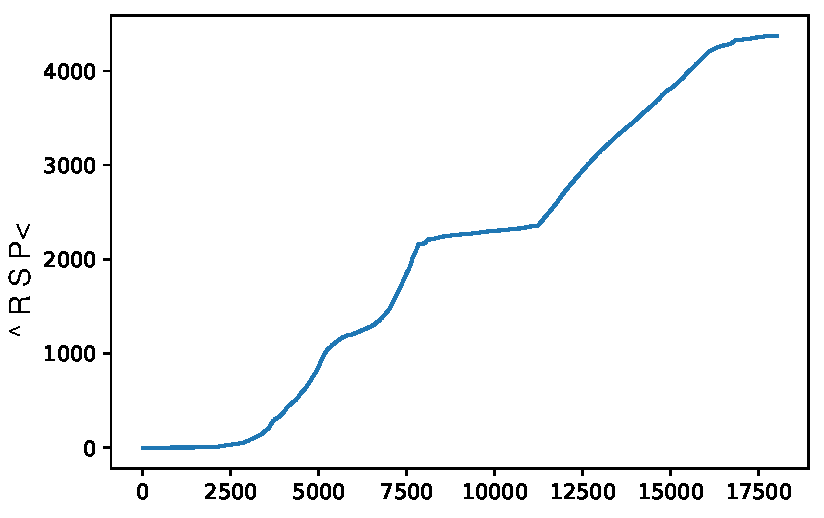
\includegraphics[width=0.4\textwidth]{Img/chapter11/align-martingale-MLPClassifier}
%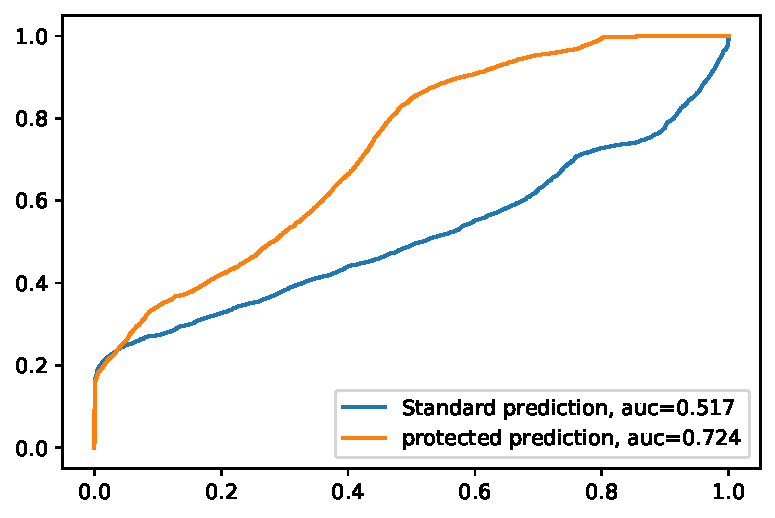
\includegraphics[width=0.4\textwidth]{Img/chapter11/align-MLPClassifier}
%\end{center}
%\caption{Align数据集的复合跳跃鞅以及鞅保护分布算法结果}
%\label{fig:align}
%\end{figure}

\begin{figure}
     \centering
     \begin{subfigure}[b]{.45\textwidth}
         \centering
         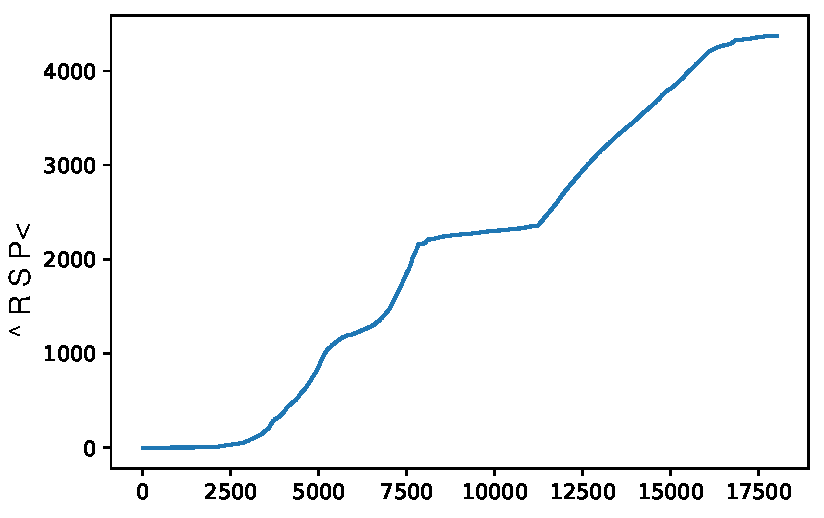
\includegraphics[width=1\textwidth]{Img/chapter11/align-martingale-MLPClassifier}   
         \caption{Align数据集的复合跳跃鞅}
         \label{mlp-jump}
     \end{subfigure}
     \hfill
     \begin{subfigure}[b]{.45\textwidth}
         \centering
         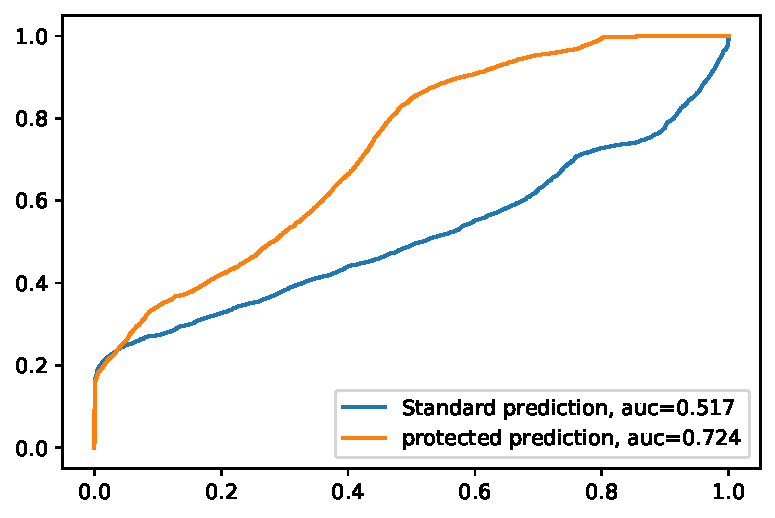
\includegraphics[width=1\textwidth]{Img/chapter11/align-MLPClassifier}
         \caption{Align数据集鞅保护分布算法结果}
         \label{mlp-jump-martingale-align}
     \end{subfigure}
\caption{Align数据集的复合跳跃鞅以及鞅保护分布算法结果}
\label{fig:align}
\end{figure}

对于Flock 数据集, 图\ref{mlp-jump-flock} 给出的是复合鞅序列, 类似的可以看到Flock数据集也发生分布漂移。 利用这种分布变化, 基于鞅保护分布算法校正底层神经网络算法。 图\ref{mlp-jump-martingale-flock} 给出校正后的ROC得分比较。 很明显, 通过鞅保护分布算法针对Flock数据集的底层神经网络的AUC值从0.63提升至0.715。 

%\begin{figure} % [tb]
%\begin{center}
%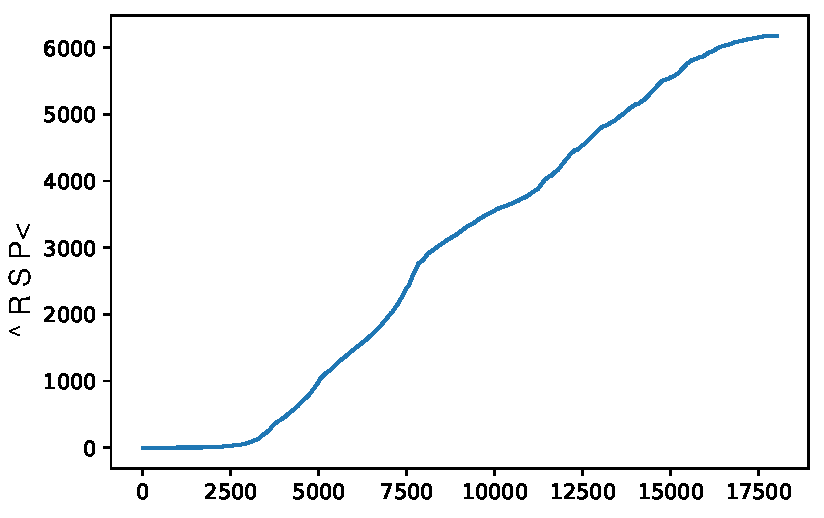
\includegraphics[width=0.4\textwidth]{Img/chapter11/flock-martingale-MLPClassifier}
%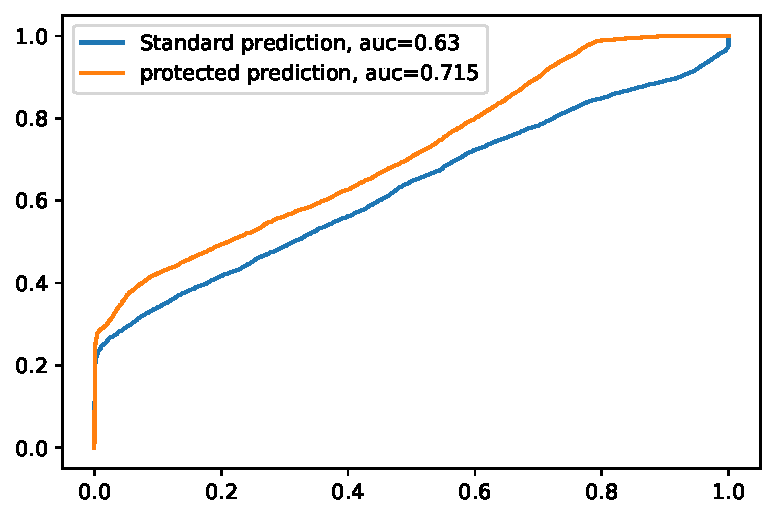
\includegraphics[width=0.4\textwidth]{Img/chapter11/flock-MLPClassifier}
%\end{center}
%\caption{Flock数据集的复合跳跃鞅以及鞅保护分布算法结果}
%\label{fig:flock}
%\end{figure}

\begin{figure}
     \centering
     \begin{subfigure}[b]{.45\textwidth}
         \centering
         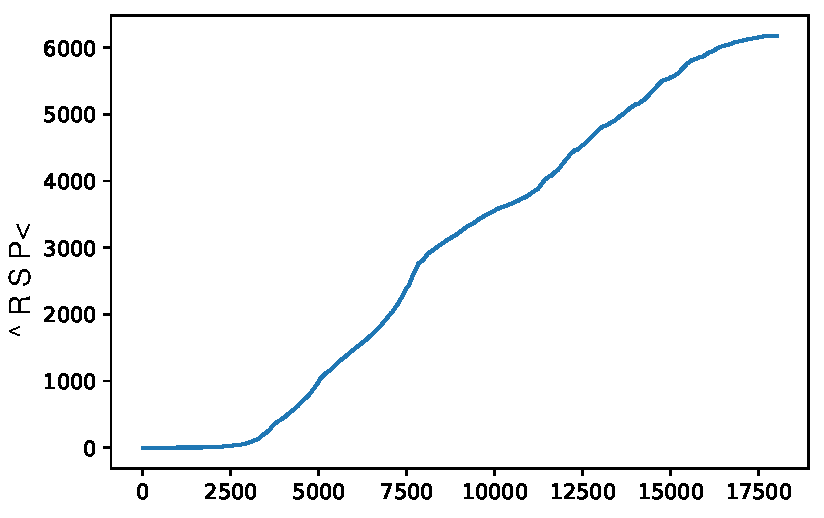
\includegraphics[width=1\textwidth]{Img/chapter11/flock-martingale-MLPClassifier}   
         \caption{Flock数据集的复合跳跃鞅}
         \label{mlp-jump-flock}
     \end{subfigure}
     \hfill
     \begin{subfigure}[b]{.45\textwidth}
         \centering
         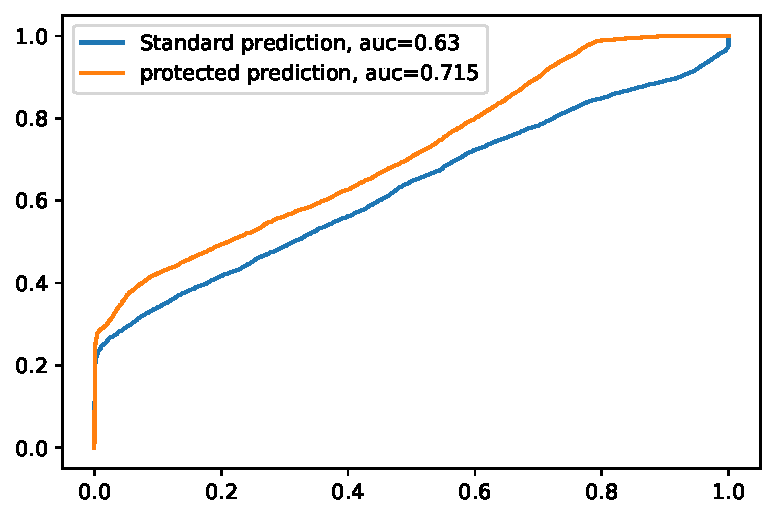
\includegraphics[width=1\textwidth]{Img/chapter11/flock-MLPClassifier}
         \caption{Flock数据集鞅保护分布算法结果}
         \label{mlp-jump-martingale-flock}
     \end{subfigure}
\caption{Flock数据集的复合跳跃鞅以及鞅保护分布算法结果}
\label{fig:flock}
\end{figure}

对于Group数据集, 图 \ref{mlp-jump-group} 给出的是复合鞅序列, 同样可以看到Group数据集也发生分布漂移。 利用这种分布变化, 基于鞅保护分布算法校正底层神经网络算法。 图\ref{mlp-jump-martingale-group} 给出校正后的ROC得分比较。 很明显, 通过鞅保护分布算法针对Group数据集分类指标AUC由神经网络算法的0.715提升至0.789。

%\begin{figure} % [tb]
%\begin{center}
%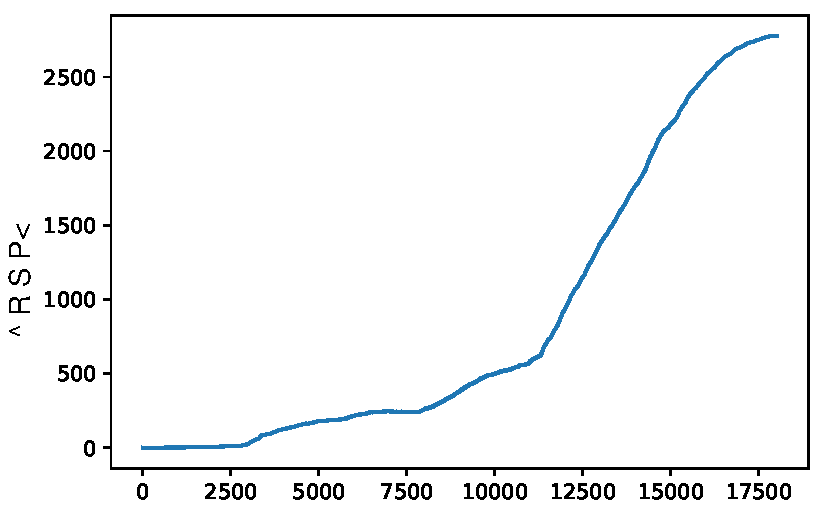
\includegraphics[width=0.4\textwidth]{Img/chapter11/group-martingale-MLPClassifier}
%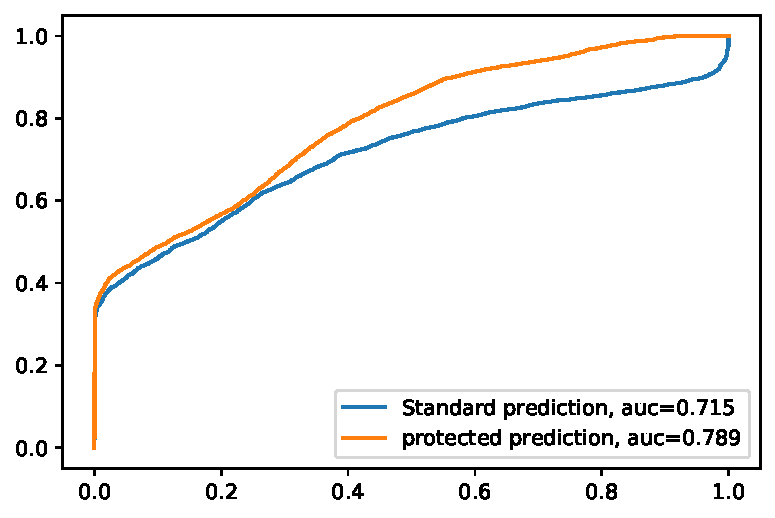
\includegraphics[width=0.4\textwidth]{Img/chapter11/group-MLPClassifier}
%\end{center}
%\caption{Group数据集的复合跳跃鞅以及鞅保护分布算法结果}
%\label{fig:group}
%\end{figure}

\begin{figure}
     \centering
     \begin{subfigure}[b]{.45\textwidth}
         \centering
         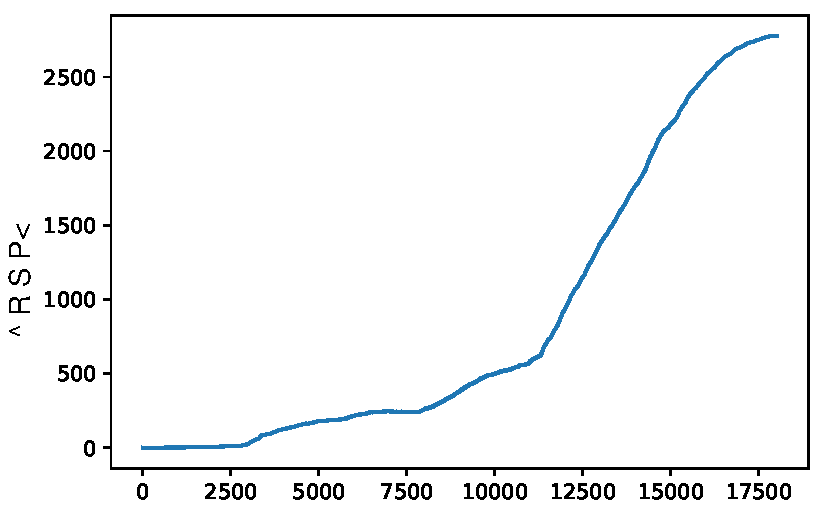
\includegraphics[width=1\textwidth]{Img/chapter11/group-martingale-MLPClassifier}   
         \caption{Group数据集的复合跳跃鞅}
         \label{mlp-jump-group}
     \end{subfigure}
     \hfill
     \begin{subfigure}[b]{.45\textwidth}
         \centering
         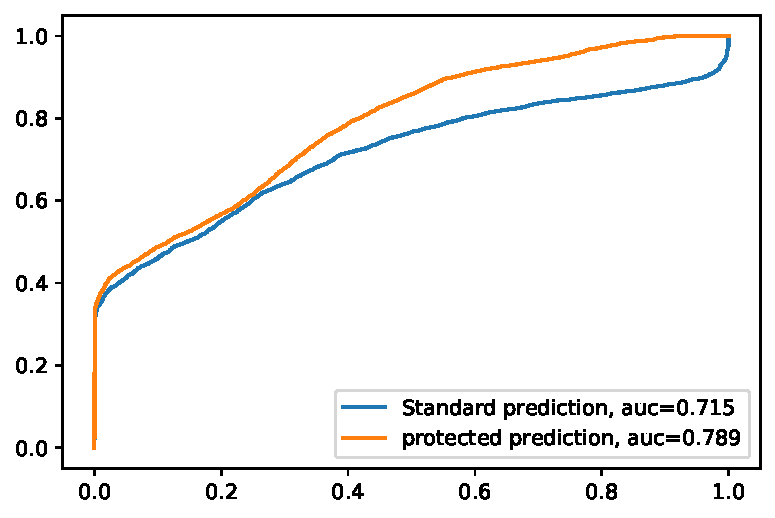
\includegraphics[width=1\textwidth]{Img/chapter11/group-MLPClassifier}
         \caption{Group数据集鞅保护分布算法结果}
         \label{mlp-jump-martingale-group}
     \end{subfigure}
\caption{Group数据集的复合跳跃鞅以及鞅保护分布算法结果}
\label{fig:group}
\end{figure}

为了和第\ref{chapter:swarm-distributions}章中讨论的结果比较, 本章给出有序学习下三种无人机集群错误分类数目的统计对比。表\ref{tab:align-num-martingale}给出Align数据集鞅保护分布算法预测错误数目与第\ref{chapter:swarm-distributions}章中表\ref{tab:online}的对比结果。从表\ref{tab:align-num-martingale}可知, 采用鞅保护分布算法能够明显降低错误分类的数目。例如, 经过鞅保护分布算法, 对于Align数据集可以将第\ref{chapter:swarm-distributions}章中表\ref{tab:online}采用SVMs算法分类错误数目由1492降低到1347, 降幅9.72\%; 将采用神经网络算法分类错误数目由848降低到665, 降幅21.58\%; 将采用Boosting算法分类错误数目由1763降低到1477, 降幅16.22\%。

% Please add the following required packages to your document preamble:
% \usepackage{booktabs}
% \usepackage{graphicx}
\begin{table}[]
\centering
\caption{Align数据集鞅保护分布算法预测错误数目对比}
\label{tab:align-num-martingale}
\begin{tabular}{@{}llll@{}}
\toprule
预测算法类别   & 无保护时错误数目(表\ref{tab:online}) & 鞅保护后错误数目 & 提升百分比 \\ \midrule
SVMs     & 1492          & \textbf{1347}      &       {9.72\%}\\
神经网络     & 848           & \textbf{665}      &     {21.58\%} \\
Boosting & 1763          & \textbf{1477}     &       {16.22\%} \\ \bottomrule
\end{tabular}%
\end{table}

表\ref{tab:flock-num-martingale}给出Flock数据集鞅保护分布算法预测错误数目与第\ref{chapter:swarm-distributions}章中表\ref{tab:online}的对比结果。对于Flock数据集可以将第\ref{chapter:swarm-distributions}章中表\ref{tab:online}采用神经网络算法分类错误数目由2125降低到1876, 降幅11.72\%; 将采用Boosting算法分类错误数目由2055降低到1742, 降幅15.23\%; 但是对于采用SVMs算法却没有给出提升效果。

% Please add the following required packages to your document preamble:
% \usepackage{booktabs}
% \usepackage{graphicx}
\begin{table}[]
\centering
\caption{Flock数据集鞅保护分布算法预测错误数目对比}
\label{tab:flock-num-martingale}
\begin{tabular}{@{}llll@{}}
\toprule
预测算法类别   & 无保护时错误数目(表\ref{tab:online}) & 鞅保护后错误数目 & 提升百分比 \\ \midrule
SVMs     & \textbf{2928}          & 3027      &       {-3.38\%}\\
神经网络     & 2125           & \textbf{1876}      &     {11.72\%}  \\
Boosting & 2055          & \textbf{1742}     &       {15.23\%} \\ \bottomrule
\end{tabular}%
\end{table}


表\ref{tab:group-num-martingale}给出Group数据集鞅保护分布算法预测错误数目与第\ref{chapter:swarm-distributions}章中表\ref{tab:online}的对比结果。对于Group数据集可以将第\ref{chapter:swarm-distributions}章中表\ref{tab:online}采用神经网络算法分类错误数目由1031降低到942, 降幅8.63\%; 将采用Boosting算法分类错误数目由452降低到401, 降幅11.28\%; 但是对于采用SVMs算法却没有给出提升效果。

% Please add the following required packages to your document preamble:
% \usepackage{booktabs}
% \usepackage{graphicx}
\begin{table}[]
\centering
\caption{Group数据集鞅保护分布算法预测错误数目对比}
\label{tab:group-num-martingale}
\begin{tabular}{@{}llll@{}}
\toprule
预测算法类别   & 无保护时错误数目(表\ref{tab:online}) & 鞅保护后错误数目 & 提升百分比 \\ \midrule
SVMs     & \textbf{1385}          & 1421      &      {-2.60\%} \\
神经网络     & 1031           & \textbf{942}      &   {8.63\%}   \\
Boosting & 452          & \textbf{401}     &      {11.28\%} \\ \bottomrule
\end{tabular}%
\end{table}


同样的, 也可以针对其他不同机器学习算法对比鞅保护分布算法的效果。分别选择 SVMs, 神经网络, 决策树模型, 随机森林, 朴素贝叶斯和逻辑回归等六种机器学习作为底层算法, 检验采用鞅保护前后的泛化推广能力。 为了统一比较算法, 本次对比选择更常用的AUC值作为评价指标。

表 \ref{tab:align} 展示的是针对Align数据集, 这六种学习算法在采用鞅保护前后的预测能力。 从表中可以看到, 对于Align数据集, 鞅保护后的算法比未经鞅保护的底层算法预测能力都得到提高。 例如, 对于常规SVMs算法, 其对于Align行为分类效果的AUC值为0.654, 采用鞅保护分布算法得到的AUC值提升至 0.732; 对于常规神经网络算法, 其对于Align行为分类效果的AUC值为0.517, 采用鞅保护分布算法得到的AUC值提升至 0.724; 对于常规决策树模型算法, 其对于Align行为分类效果的AUC值为0.508, 采用鞅保护分布算法得到的AUC值提升至 0.641; 对于常规随机森林算法, 其对于Align行为分类效果的AUC值为0.604, 采用鞅保护分布算法得到的AUC值提升至 0.722; 对于常规朴素贝叶斯算法, 其对于Align行为分类效果的AUC值为0.460, 采用鞅保护分布算法得到的AUC值提升至 0.650; 对于常规逻辑回归算法, 其对于Align行为分类效果的AUC值为0.440, 采用鞅保护分布算法得到的AUC值提升至 0.710。 并且通过这种对比可以看到, 鞅保护分布算法对于基于模型假定的传统统计学范式(朴素贝叶斯和逻辑回归模型)的提升能力是相当明显可观的。 

% Please add the following required packages to your document preamble:
% \usepackage{booktabs}
\begin{table}[]
\centering
\caption{Align数据集鞅保护分布算法对比汇总表}
\label{tab:align}
\begin{tabular}{@{}llll@{}}
\toprule
预测算法类别 & 无保护时AUC值 & 鞅保护后AUC值 & 提升百分比 \\ \midrule
SVMs                & 0.654     & \textbf{0.732}  &  {10.66\%}  \\
神经网络       & 0.517     & \textbf{0.724}  &  {28.59\%}  \\
决策树        & 0.508     & \textbf{0.641}  &  {20.75\%} \\
随机森林        & 0.604     & \textbf{0.722}  &  {16.34\%} \\
朴素贝叶斯     & 0.460     & \textbf{0.650}  &  {29.23\%}  \\
逻辑回归  & 0.440     & \textbf{0.710}  &  {38.03\%}  \\ \bottomrule
\end{tabular}
\end{table}

表 \ref{tab:flock} 给出针对 Flock 数据集的预测效果对比。 从表中可以看到, 对于常规SVMs算法, 其对于Flock行为分类效果的AUC值为0.749, 采用鞅保护分布算法得到的AUC值降低为 0.721; 对于常规神经网络算法, 其对于Flock行为分类效果的AUC值为0.630, 采用鞅保护分布算法得到的AUC值提升至 0.715; 对于常规决策树模型算法, 其对于Flock行为分类效果的AUC值为0.654, 采用鞅保护分布算法得到的AUC值提升至 0.703; 对于常规随机森林算法, 其对于Flock行为分类效果的AUC值为0.707, 采用鞅保护分布算法得到的AUC值提升至 0.814; 对于常规朴素贝叶斯算法, 其对于Flock行为分类效果的AUC值为0.627, 采用鞅保护分布算法得到的AUC值提升至 0.687; 对于常规逻辑回归算法, 其对于Flock行为分类效果的AUC值为0.598, 采用鞅保护分布算法得到的AUC值提升至 0.694。 当然在Flock数据集上, 鞅保护分布算法对于SVMs算法并没有带来分类能力的提升, 反而降低其AUC值。 这是因为对于SVMs算法, 由于其本身属于超越推理模型, 其输出值并不来自最外层固定的具体函数。 因此可以理解为什么在Flock数据集上鞅保护分布算法对SVMs给出相反的结论。

% Please add the following required packages to your document preamble:
% \usepackage{booktabs}
\begin{table}[]
\centering
\caption{Flock数据集鞅保护分布算法对比汇总表}
\label{tab:flock}
\begin{tabular}{@{}llll@{}}
\toprule
预测算法类别 & 无保护时AUC值 & 鞅保护后AUC值 & 提升百分比 \\ \midrule
SVMs                 & \textbf{0.749}        & 0.721      		 & {-3.88\%}\\
神经网络       & 0.630                 & \textbf{0.715}      & {11.89\%}\\
决策树        & 0.654                 & \textbf{0.703}      & {6.67\%}\\
随机森林        & 0.707                 & \textbf{0.814}      & {13.14\%}\\
朴素贝叶斯     & 0.627                 & \textbf{0.687}      & {8.73\%}\\
逻辑回归  & 0.598                 & \textbf{0.694}      & {13.83\%}\\ \bottomrule
\end{tabular}
\end{table}

鞅保护分布算法为底层机器学习算法带来的提升在Group数据集上也具有明显的提升效果。 表 \ref{tab:group} 展示的是这六种算法以及对应的鞅保护分布算法对Group行为数据集学习效果提升的对比。从表中可以看到, 对于常规SVMs算法, 其对于Group行为分类效果的AUC值为0.827, 采用鞅保护分布算法得到的AUC值降低为 0.809; 对于常规神经网络算法, 其对于Group行为分类效果的AUC值为0.715, 采用鞅保护分布算法得到的AUC值提升至 0.789; 对于常规决策树模型算法, 其对于Group行为分类效果的AUC值为0.545, 采用鞅保护分布算法得到的AUC值提升至 0.654; 对于常规随机森林算法, 其对于Group行为分类效果的AUC值为0.686, 采用鞅保护分布算法得到的AUC值提升至 0.784; 对于常规朴素贝叶斯算法, 其对于Group行为分类效果的AUC值为0.693, 采用鞅保护分布算法得到的AUC值提升至 0.746; 对于常规逻辑回归算法, 其对于Group行为分类效果的AUC值为0.731, 采用鞅保护分布算法得到的AUC值提升至 0.789。 同样的, 在Group行为数据集合上, 鞅保护分布算法对于SVMs模型并没有给出提升的效果, 但是对于其他机器学习算法, 其均给出令人满意的结果。

% Please add the following required packages to your document preamble:
% \usepackage{booktabs}
\begin{table}[]
\centering
\caption{Group数据集鞅保护分布算法对比汇总表}
\label{tab:group}
\begin{tabular}{@{}llll@{}}
\toprule
预测算法类别 & 无保护时AUC值 & 鞅保护后AUC值 & 提升百分比\\ \midrule
SVMs                 & \textbf{0.827}        & 0.809               & {-2.22\%}\\
神经网络      & 0.715                 & \textbf{0.789}      & {9.38\%}\\
决策树       & 0.545                 & \textbf{0.654}      & {16.67\%}\\
随机森林        & 0.686                 & \textbf{0.784}      & {12.50\%}\\
朴素贝叶斯     & 0.693                 & \textbf{0.746}      & {7.10\%}\\
逻辑回归  & 0.731                 & \textbf{0.789}      & {7.35\%}\\ \bottomrule
\end{tabular}
\end{table}
 
\section{本章小结}
\label{conclusion}
本章以无人机集群行为数据本身的时间顺序为研究对象, 针对考虑数据自身时间顺序的无人机集群行为分类问题进行研究。主要结论总结如下:
\begin{enumerate}
\item 针对实际工程应用中数据可能出现的分布漂移现象, 构建新的分布漂移检测指标。这种新检测指标同样也能够高效地给出分布漂移的证据;
\item 提出一种鞅保护分布框架提升底层机器学习算法的性能。鞅保护分布算法建立在机器学习算法顶层, 可以为大多数机器学习算法的预测效果提供明显的改进;
\item 本节提出的算法不仅仅指出实际数据中会出现的分布漂移现象, 而且将数据本身的分布信息融合至底层学习算法, 说明数据本身的时间顺序是不可被忽视的信息。
\end{enumerate}